\documentclass[preprint,12pt,aps,pra,showkeys,amsmath,amssymb,superscriptaddress,floatfix]{revtex4-2}
\usepackage[T1]{fontenc}
\usepackage[utf8]{inputenc}
\usepackage{amsmath,amssymb,amsthm,mathtools,mathrsfs}
\usepackage{microtype,booktabs,enumitem}
\usepackage{xcolor,tikz,etoolbox}
\usepackage[skins,breakable]{tcolorbox}
\usepackage{needspace}
% Keep diagram geometry independent of REVTeX preprint body spacing.
\AtBeginEnvironment{tikzpicture}{\linespread{1}\selectfont}
\usetikzlibrary{arrows.meta,positioning,calc,fit,decorations.pathreplacing}
\usepackage{graphicx}
\usepackage{hyperref}

\definecolor{MMBlue}{RGB}{0,82,155}
\definecolor{MMOrange}{RGB}{200,80,0}
\tikzset{
 mmnode/.style={draw=MMBlue,rounded corners=2pt,fill=MMBlue!4,align=left,execute at begin node={\raggedright},text width=5cm,font=\fontsize{10}{12}\selectfont,inner sep=6pt},
 mmimport/.style={mmnode,draw=black!65,fill=black!4},
 mmcandidate/.style={mmnode,draw=MMOrange,dashed,fill=MMOrange!5},
 mmrejected/.style={mmnode,draw=black,densely dotted,fill=black!8},
 mmproof/.style={->,thick,MMBlue},
 mmflow/.style={->,semithick,black!70},
 mmrepair/.style={->,dashed,thick,MMOrange},
 mmcandidatearrow/.style={->,dashed,semithick,MMOrange},
 mmnote/.style={font=\scriptsize,fill=white,inner sep=2pt,align=center}}

\usepackage[section]{placeins}
\setlength{\emergencystretch}{3em}
\setlist{itemsep=3pt,topsep=4pt}
\newtheorem{theorem}{Theorem}[section]
\newtheorem{proposition}[theorem]{Proposition}
\newtheorem{lemma}[theorem]{Lemma}
\newtheorem{corollary}[theorem]{Corollary}
\theoremstyle{definition}
\newtheorem{definition}[theorem]{Definition}
\newtheorem{example}[theorem]{Example}
\theoremstyle{remark}
\newtheorem{remark}[theorem]{Remark}
% Avoid isolated statement headings and single-line paragraph fragments.
\BeforeBeginEnvironment{theorem}{\Needspace{6\baselineskip}}
\BeforeBeginEnvironment{definition}{\Needspace{5\baselineskip}}
\BeforeBeginEnvironment{proposition}{\Needspace{5\baselineskip}}
\BeforeBeginEnvironment{lemma}{\Needspace{5\baselineskip}}
\BeforeBeginEnvironment{corollary}{\Needspace{5\baselineskip}}
\clubpenalty=5000
\widowpenalty=5000
\newcommand{\R}{\mathbb R}\newcommand{\Z}{\mathbb Z}\newcommand{\N}{\mathbb N}
\newcommand{\Pa}{\operatorname{Pa}}\newcommand{\Desc}{\operatorname{Desc}}
\newcommand{\cl}{\operatorname{cl}}\newcommand{\cost}{\operatorname{cost}}
\newcommand{\status}{\operatorname{status}}
% Faculty cards: a visual rail groups the five faculties within one agent.
% The rail has no arrowhead and does not represent a proof dependency.
\newcommand{\mmfacultybadge}[1]{%
 \node[circle,draw=MMBlue,line width=1pt,fill=white,
 minimum size=7mm,inner sep=0pt,font=\sffamily\small\bfseries,text=MMBlue]
 at ([xshift=15pt,yshift=-15pt]frame.north west) {#1};}
\newcommand{\mmfacultyrail}{%
 \draw[MMBlue!80,line width=1pt]
 ([xshift=15pt,yshift=2pt]frame.north west)--
 ([xshift=15pt,yshift=-2pt]frame.south west);}
\newtcolorbox{mmfacultybox}[2]{enhanced,breakable,
 colback=MMBlue!4,colframe=MMBlue!4,boxrule=0pt,arc=3pt,
 left=39pt,right=9pt,top=4pt,bottom=4pt,
 before skip=2pt,after skip=2pt,
 fontupper=\small\linespread{1.1}\selectfont,
 overlay unbroken={\mmfacultyrail\mmfacultybadge{#1}},
 overlay first={\mmfacultyrail\mmfacultybadge{#1}},
 overlay middle={\mmfacultyrail},overlay last={\mmfacultyrail}}
\newcommand{\mmfaculty}[3]{%
 \begin{mmfacultybox}{#1}{#2}
 {\sffamily\bfseries\color{MMBlue}#2}\par\smallskip #3
 \end{mmfacultybox}}
\newcommand{\agent}[9]{%
 \Needspace{8\baselineskip}
 \subsubsection{#1}
 \noindent\textbf{Object.} #2\par
 \noindent\textbf{Role.} #3\par\smallskip
 \mmfaculty{E}{Ego}{#4}
 \mmfaculty{M}{Memory}{#5}
 \mmfaculty{I}{Intellect}{#6}
 \mmfaculty{S}{Sense}{#7}
 \mmfaculty{A}{Action}{#8}
 \smallskip\noindent #9\par}

\usepackage{longtable,array,calc}
\providecommand{\tightlist}{\setlength{\itemsep}{2pt}\setlength{\parskip}{0pt}}
\makeatletter
\def\frontmatter@abstract@produce{\par\addvspace{\frontmatter@preabstractspace}%
\begingroup\prep@absbox\unvbox\absbox\post@absbox\endgroup
\addvspace{\frontmatter@postabstractspace}}
\makeatother
\newcommand{\field}[2]{\par\smallskip\noindent\textbf{#1.} #2\par}
\setlength{\emergencystretch}{5em}
\AtBeginEnvironment{verbatim}{\small\linespread{1.0}\selectfont}


\hypersetup{colorlinks=true,linkcolor=MMBlue,urlcolor=MMBlue,pdfauthor={Dibakar Sigdel}}

\begin{document}

\title{Lie's Theorem for Solvable Complex Lie Algebras\\[4pt]\large An End-to-End Meta-Math Walkthrough}

\author{Dibakar Sigdel}

\affiliation{Mindverse Computing LLC, Lynnwood, WA 98087, USA}

\date{October 2026}

\begin{abstract}

An ideal of codimension one provides a weight vector by induction. A
trace calculation prevents the remaining direction from changing that
weight, enabling one last eigenvector selection. The report presents the
target theorem, declared imports, a dependency graph, five-faculty node
contracts, a continuous proof, a worked example, and a hypothesis-repair
audit. It is an authored mathematical exposition, not a deployed-agent
transcript or a formal proof-assistant certificate.

\end{abstract}\maketitle\linespread{1.12}\selectfont

\noindent\textbf{RT-04 / Representation Theory and Lie Theory / Report v1}

\section{Target and import contract}

\begin{theorem}

Let \(\mathfrak g\) be a finite-dimensional solvable complex Lie algebra
and \(\rho:\mathfrak g\to\mathfrak{gl}(V)\) a representation on a
nonzero finite-dimensional complex vector space. There is a common
eigenvector: some \(v\ne0\) and linear
\(\lambda:\mathfrak g\to\mathbb C\) satisfy \(\rho(y)v=\lambda(y)v\) for
all \(y\). Consequently there is a basis in which every \(\rho(y)\) is
upper triangular. Solvable means the iterated derived series eventually
becomes zero.

\end{theorem}

\subsection{Foundations and permitted imports}

Use eigenvalue existence over \(\mathbb C\), trace of a commutator equal
to zero, induction on dimension, and the representation identity
\(\rho([x,y])=[\rho(x),\rho(y)]\). Write \(yv\) for \(\rho(y)v\). A
subalgebra of a solvable algebra is solvable. A nonzero solvable algebra
has \([\mathfrak g,\mathfrak g]\ne\mathfrak g\), since equality would
make its derived series constant and nonzero.

\clearpage\section{Node interaction workflow}

\begin{center}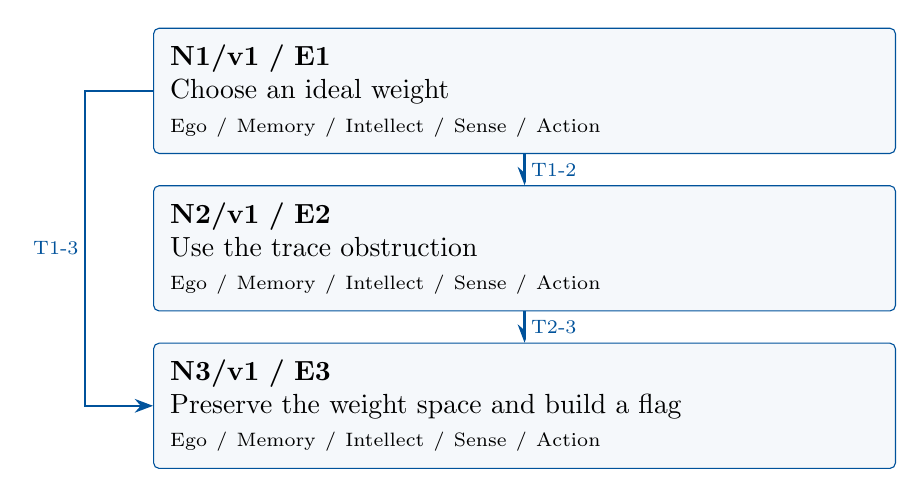
\begin{tikzpicture}[>=Stealth,x=1cm,y=1cm]

\node[mmnode,text width=9cm,minimum height=1.25cm] (N1) at (0,0.0) {\textbf{N1/v1 / E1}\\Choose an ideal weight\\{\scriptsize Ego / Memory / Intellect / Sense / Action}};

\node[mmnode,text width=9cm,minimum height=1.25cm] (N2) at (0,-2.0) {\textbf{N2/v1 / E2}\\Use the trace obstruction\\{\scriptsize Ego / Memory / Intellect / Sense / Action}};

\node[mmnode,text width=9cm,minimum height=1.25cm] (N3) at (0,-4.0) {\textbf{N3/v1 / E3}\\Preserve the weight space and build a flag\\{\scriptsize Ego / Memory / Intellect / Sense / Action}};

\draw[mmproof] (N1.south) -- node[mmnote,right] {T1-2} (N2.north);

\draw[mmproof] (N1.west) -- (-5.58,0) -- node[mmnote,left] {T1-3} (-5.58,-4) -- (N3.west);

\draw[mmproof] (N2.south) -- node[mmnote,right] {T2-3} (N3.north);

\end{tikzpicture}\end{center}

Each box is one mathematical agent containing all five faculties. Blue
arrows carry the versioned exports listed below. The layout gives a
reading order; only drawn arrows assert dependencies. Diagnostic repair
is separate from the proof DAG.

\subsection{Versioned evidence-transfer ledger}

\begingroup\small\linespread{1.05}\selectfont

\Needspace{5\baselineskip}\field{T1-2: N1/E1/v1 to N2}{There exist \(x\) with \(\mathfrak g=\mathfrak h\oplus\mathbb Cx\), a
nonzero \(v_0\), and a linear weight \(\lambda\) on \(\mathfrak h\) with
\(yv_0=\lambda(y)v_0\).}

\field{Receiving activity}{N2.1}

\field{Compatibility}{E1/v1 and \(W=\operatorname{span}\{v_0,xv_0,x^2v_0,\ldots\}\). Check:
The finite span \(W\) is invariant under both \(x\) and \(\mathfrak h\),
so restricted commutator traces are legitimate.}

\Needspace{5\baselineskip}\field{T1-3: N1/E1/v1 to N3}{There exist \(x\) with \(\mathfrak g=\mathfrak h\oplus\mathbb Cx\), a
nonzero \(v_0\), and a linear weight \(\lambda\) on \(\mathfrak h\) with
\(yv_0=\lambda(y)v_0\).}

\field{Receiving activity}{N3.1}

\field{Compatibility}{E1/v1 and E2/v1;
\(E=\{v:yv=\lambda(y)v\text{ for all }y\in\mathfrak h\}\). Check:
\(E\ne0\) since it contains \(v_0\); the final induction decreases
representation dimension.}

\Needspace{5\baselineskip}\field{T2-3: N2/E2/v1 to N3}{\(\lambda([x,y])=0\) for every \(y\in\mathfrak h\).}

\field{Receiving activity}{N3.1}

\field{Compatibility}{E1/v1 and E2/v1;
\(E=\{v:yv=\lambda(y)v\text{ for all }y\in\mathfrak h\}\). Check:
\(E\ne0\) since it contains \(v_0\); the final induction decreases
representation dimension.}

\endgroup

\clearpage\section{Agent roles and five-faculty activities}\begingroup\small\linespread{1.05}\selectfont\setlist{itemsep=1pt,topsep=2pt}

\subsection{N1/v1: Choose an ideal weight}

\field{Object and role}{Reduce the Lie algebra dimension, then record the orbit of a weight
vector under the missing direction. \textbf{Local obligation:} There
exist \(x\) with \(\mathfrak g=\mathfrak h\oplus\mathbb Cx\), a nonzero
\(v_0\), and a linear weight \(\lambda\) on \(\mathfrak h\) with
\(yv_0=\lambda(y)v_0\).}

\field{Inputs}{Induction on \(d=\dim\mathfrak g\) and a hyperplane
\(\mathfrak h\supset[\mathfrak g,\mathfrak g]\).}

\mmfaculty{E}{Ego}{Publish E1/v1 only after establishing this obligation: There exist \(x\)
with \(\mathfrak g=\mathfrak h\oplus\mathbb Cx\), a nonzero \(v_0\), and
a linear weight \(\lambda\) on \(\mathfrak h\) with
\(yv_0=\lambda(y)v_0\).}

\mmfaculty{M}{Memory}{Induction on \(d=\dim\mathfrak g\) and a hyperplane
\(\mathfrak h\supset[\mathfrak g,\mathfrak g]\). Retain the stated
assumptions and import versions.}

\mmfaculty{I}{Intellect}{Reduce the Lie algebra dimension, then record the orbit of a weight
vector under the missing direction.}

\mmfaculty{S}{Sense}{\(\mathfrak h\) is an ideal because every bracket with it lies in
\([\mathfrak g,\mathfrak g]\); induction decreases algebra dimension.}

\mmfaculty{A}{Action}{Carry out activities N1.1--N1.2 below, retaining each calculation and
construction as evidence.}

\smallskip\noindent\textbf{Numbered mathematical activities}

\begin{enumerate}[label=N1.\arabic*,leftmargin=3.4em]

\item When \(\mathfrak g=0\), any nonzero vector works. For \(d>0\),
solvability makes the derived algebra proper. Choose a hyperplane
\(\mathfrak h\) containing it and \(x\) outside. The hyperplane is an
ideal and solvable, of dimension \(d-1\).

\item Apply the induction hypothesis to the restriction of the representation
to \(\mathfrak h\). It gives \(v_0\ne0\) with \(yv_0=\lambda(y)v_0\).
The scalar function \(\lambda\) is linear because the representation is
linear and \(v_0\) is nonzero.

\end{enumerate}

\field{Export E1/v1}{There exist \(x\) with \(\mathfrak g=\mathfrak h\oplus\mathbb Cx\), a
nonzero \(v_0\), and a linear weight \(\lambda\) on \(\mathfrak h\) with
\(yv_0=\lambda(y)v_0\).}

\field{Acceptance gate}{\(\mathfrak h\) is an ideal because every bracket with it lies in
\([\mathfrak g,\mathfrak g]\); induction decreases algebra dimension.}

\field{Targeted repair}{If an arbitrary hyperplane is assumed ideal, choose one containing the
derived algebra before applying the commutator calculation. Withhold
this export and recheck its descendants after a versioned correction.}

\clearpage

\subsection{N2/v1: Use the trace obstruction}

\field{Object and role}{Triangularize the ideal action on a finite cyclic span and take traces
of commutators there. \textbf{Local obligation:} \(\lambda([x,y])=0\)
for every \(y\in\mathfrak h\).}

\field{Inputs}{E1/v1 and \(W=\operatorname{span}\{v_0,xv_0,x^2v_0,\ldots\}\). Incoming
proof exports: E1/v1 at N2.1.}

\mmfaculty{E}{Ego}{Publish E2/v1 only after establishing this obligation:
\(\lambda([x,y])=0\) for every \(y\in\mathfrak h\).}

\mmfaculty{M}{Memory}{E1/v1 and \(W=\operatorname{span}\{v_0,xv_0,x^2v_0,\ldots\}\). Incoming
proof exports: E1/v1 at N2.1. Retain the stated assumptions and import
versions.}

\mmfaculty{I}{Intellect}{Triangularize the ideal action on a finite cyclic span and take traces
of commutators there.}

\mmfaculty{S}{Sense}{The finite span \(W\) is invariant under both \(x\) and \(\mathfrak h\),
so restricted commutator traces are legitimate.}

\mmfaculty{A}{Action}{Carry out activities N2.1--N2.3 below, retaining each calculation and
construction as evidence.}

\smallskip\noindent\textbf{Numbered mathematical activities}

\begin{enumerate}[label=N2.\arabic*,leftmargin=3.4em]

\item Put \(v_j=x^jv_0\). Induction on \(j\), simultaneously for every
\(y\in\mathfrak h\), gives
\(yv_j-\lambda(y)v_j\in\operatorname{span}(v_0,\ldots,v_{j-1})\). Indeed
\(yxv_{j-1}=x(yv_{j-1})+[y,x]v_{j-1}\); the first term has the required
leading part and the second lies in the previous span because
\([y,x]\in\mathfrak h\) and the induction hypothesis applies to it.

\item Let \(m\ge1\) be the first index where \(v_m\) depends on its
predecessors. It exists by finite dimension. Then \(v_0,\ldots,v_{m-1}\)
form a basis of \(W\), which is \(x\)-invariant and, by the preceding
formula, \(\mathfrak h\)-invariant. For \(y\in\mathfrak h\), its action
on \(W\) is triangular with all diagonal entries \(\lambda(y)\).

\item The action of \([x,y]\) on \(W\) is the commutator of the two restricted
operators, so its trace is zero. It also has trace \(m\lambda([x,y])\),
since \([x,y]\in\mathfrak h\). Characteristic zero gives
\(\lambda([x,y])=0\).

\end{enumerate}

\field{Export E2/v1}{\(\lambda([x,y])=0\) for every \(y\in\mathfrak h\).}

\field{Acceptance gate}{The finite span \(W\) is invariant under both \(x\) and \(\mathfrak h\),
so restricted commutator traces are legitimate.}

\field{Targeted repair}{If a trace is taken on a noninvariant partial span, first pass to the
full finite cyclic space \(W\) and establish both invariances. Withhold
this export and recheck its descendants after a versioned correction.}

\clearpage

\subsection{N3/v1: Preserve the weight space and build a flag}

\field{Object and role}{Use the vanished commutator weights to show \(xE\subset E\), then repeat
on quotient spaces. \textbf{Local obligation:} A common eigenvector
exists, and the representation admits a full invariant flag and
upper-triangular matrices.}

\field{Inputs}{E1/v1 and E2/v1;
\(E=\{v:yv=\lambda(y)v\text{ for all }y\in\mathfrak h\}\). Incoming
proof exports: E1/v1 at N3.1, E2/v1 at N3.1.}

\mmfaculty{E}{Ego}{Publish E3/v1 only after establishing this obligation: A common
eigenvector exists, and the representation admits a full invariant flag
and upper-triangular matrices.}

\mmfaculty{M}{Memory}{E1/v1 and E2/v1;
\(E=\{v:yv=\lambda(y)v\text{ for all }y\in\mathfrak h\}\). Incoming
proof exports: E1/v1 at N3.1, E2/v1 at N3.1. Retain the stated
assumptions and import versions.}

\mmfaculty{I}{Intellect}{Use the vanished commutator weights to show \(xE\subset E\), then repeat
on quotient spaces.}

\mmfaculty{S}{Sense}{\(E\ne0\) since it contains \(v_0\); the final induction decreases
representation dimension.}

\mmfaculty{A}{Action}{Carry out activities N3.1--N3.2 below, retaining each calculation and
construction as evidence.}

\smallskip\noindent\textbf{Numbered mathematical activities}

\begin{enumerate}[label=N3.\arabic*,leftmargin=3.4em]

\item For \(v\in E\) and \(y\in\mathfrak h\),
\(y(xv)=x(yv)+[y,x]v=\lambda(y)xv+\lambda([y,x])v=\lambda(y)xv\). Thus
\(xE\subset E\). On this nonzero finite-dimensional complex space, \(x\)
has an eigenvector \(v\). Since \(\mathfrak g=\mathfrak h+\mathbb Cx\),
it is a common eigenvector for all of \(\mathfrak g\), completing the
induction on \(d\).

\item The line \(\mathbb Cv\) is invariant. To triangularize, induct
separately on \(\dim V\): the quotient \(V/\mathbb Cv\) has a
representation of the same solvable algebra and a full invariant flag by
induction. Lift its flag and prepend \(\mathbb Cv\). A basis adapted to
this flag makes all representing matrices upper triangular.

\end{enumerate}

\field{Export E3/v1}{A common eigenvector exists, and the representation admits a full
invariant flag and upper-triangular matrices.}

\field{Acceptance gate}{\(E\ne0\) since it contains \(v_0\); the final induction decreases
representation dimension.}

\field{Targeted repair}{If \(E\) is claimed invariant without E2, restore the commutator term
and use its zero weight; otherwise the eigenvector argument is
unsupported. Withhold this export and recheck its descendants after a
versioned correction.}

\endgroup\clearpage\section{Continuous mathematical proof}\label{sec:proof}

\subsection{N1 --- Choose an ideal
weight}\label{n1-choose-an-ideal-weight}

\begin{enumerate}
\def\labelenumi{\arabic{enumi}.}
\item
  \textbf{N1.1.} When \(\mathfrak g=0\), any nonzero vector works. For
  \(d>0\), solvability makes the derived algebra proper. Choose a
  hyperplane \(\mathfrak h\) containing it and \(x\) outside. The
  hyperplane is an ideal and solvable, of dimension \(d-1\).
\item
  \textbf{N1.2.} Apply the induction hypothesis to the restriction of
  the representation to \(\mathfrak h\). It gives \(v_0\ne0\) with
  \(yv_0=\lambda(y)v_0\). The scalar function \(\lambda\) is linear
  because the representation is linear and \(v_0\) is nonzero.
\end{enumerate}

\subsection{N2 --- Use the trace
obstruction}\label{n2-use-the-trace-obstruction}

\begin{enumerate}
\def\labelenumi{\arabic{enumi}.}
\item
  \textbf{N2.1.} Put \(v_j=x^jv_0\). Induction on \(j\), simultaneously
  for every \(y\in\mathfrak h\), gives
  \(yv_j-\lambda(y)v_j\in\operatorname{span}(v_0,\ldots,v_{j-1})\).
  Indeed \(yxv_{j-1}=x(yv_{j-1})+[y,x]v_{j-1}\); the first term has the
  required leading part and the second lies in the previous span because
  \([y,x]\in\mathfrak h\) and the induction hypothesis applies to it.
\item
  \textbf{N2.2.} Let \(m\ge1\) be the first index where \(v_m\) depends
  on its predecessors. It exists by finite dimension. Then
  \(v_0,\ldots,v_{m-1}\) form a basis of \(W\), which is \(x\)-invariant
  and, by the preceding formula, \(\mathfrak h\)-invariant. For
  \(y\in\mathfrak h\), its action on \(W\) is triangular with all
  diagonal entries \(\lambda(y)\).
\item
  \textbf{N2.3.} The action of \([x,y]\) on \(W\) is the commutator of
  the two restricted operators, so its trace is zero. It also has trace
  \(m\lambda([x,y])\), since \([x,y]\in\mathfrak h\). Characteristic
  zero gives \(\lambda([x,y])=0\).
\end{enumerate}

\subsection{N3 --- Preserve the weight space and build a
flag}\label{n3-preserve-the-weight-space-and-build-a-flag}

\begin{enumerate}
\def\labelenumi{\arabic{enumi}.}
\item
  \textbf{N3.1.} For \(v\in E\) and \(y\in\mathfrak h\),
  \(y(xv)=x(yv)+[y,x]v=\lambda(y)xv+\lambda([y,x])v=\lambda(y)xv\). Thus
  \(xE\subset E\). On this nonzero finite-dimensional complex space,
  \(x\) has an eigenvector \(v\). Since
  \(\mathfrak g=\mathfrak h+\mathbb Cx\), it is a common eigenvector for
  all of \(\mathfrak g\), completing the induction on \(d\).
\item
  \textbf{N3.2.} The line \(\mathbb Cv\) is invariant. To triangularize,
  induct separately on \(\dim V\): the quotient \(V/\mathbb Cv\) has a
  representation of the same solvable algebra and a full invariant flag
  by induction. Lift its flag and prepend \(\mathbb Cv\). A basis
  adapted to this flag makes all representing matrices upper triangular.
\end{enumerate}

\hfill$\square$

\section{Worked orchestration}

Let \(\mathfrak g\) be the upper-triangular \(2\times2\) complex
matrices acting on \(\mathbb C^2\). Its derived algebra consists of
strictly upper-triangular matrices, whose mutual brackets vanish, so it
is solvable. The vector \(e_1\) is a common eigenvector with weight
\(\lambda\bigl(\begin{smallmatrix}a&b\\0&d\end{smallmatrix}\bigr)=a\).
The invariant flag is \(0\subset\mathbb Ce_1\subset\mathbb C^2\).

\subsection{Boundary and hypothesis audit}

The standard representation of \(\mathfrak{sl}_2(\mathbb C)\) has no
common eigenvector: the raising matrix kills only \(\mathbb Ce_1\),
whereas the lowering matrix sends \(e_1\) to \(e_2\). This Lie algebra
is not solvable. Over \(\mathbb R\), even a one-dimensional abelian
algebra can act by a rotation without a real eigenvector.

\section{Illustrative failure and repair}

The following is an authored diagnostic scenario. Changed assumptions
define a new contract; they do not retroactively prove the original
statement.

\subsection{Rejected argument, diagnosis, and correction}
\textbf{Rejected N3 step:} the \(\mathfrak h\)-weight space is
automatically invariant under \(x\). The identity
\(y(xv)=\lambda(y)xv+\lambda([y,x])v\) exposes the missing term.
\textbf{Diagnosis:} Intellect omitted the trace obstruction.
\textbf{Repair:} establish N2 on the invariant cyclic span, then
substitute \(\lambda([y,x])=0\). This fills a genuine logical gap under
the original hypotheses; recheck the common eigenvector and flag
exports.

\subsection{Publication and reuse}
The corrected export retains its explicit assumptions. A hypothetical
revision receives a new version, and each consuming activity is
rechecked; this scenario is not a recorded runtime event. \textbf{Next
direction:} Compare this invariant-flag theorem with the highest-weight
structure of nonsolvable \(\mathfrak{sl}_2\) in RT-05.

\par\medskip\begingroup\small\linespread{1.0}\selectfont\noindent\textbf{Provenance.} This authored proof is complete relative to its declared imports. Reuse
each export with its assumptions, proof, and version. The original
Markdown remains available for comparison.
\par\endgroup

\par\smallskip\begingroup\small\linespread{1.0}\selectfont\noindent\textbf{Further reading.} \href{https://math.mit.edu/~etingof/reprbook.pdf}{Etingof and
collaborators, Introduction to Representation Theory}, sections on
representations, characters, and \(\mathfrak{sl}_2\);
\href{https://ocw.mit.edu/courses/18-745-lie-groups-and-lie-algebras-i-fall-2020/lists/lecture-notes/}{MIT
Lie Groups and Lie Algebras I lecture notes} for solvable Lie algebras.\par\endgroup

\end{document}
